
\graphicspath{{mammle/}}

\chapter{MAMMLE: phylogeny estimation based on \underline{m}ultiobjective \underline{a}pplication-aware \underline{M}USCLE and \underline{m}aximum \underline{l}ikelihood \underline{e}nsemble} \label{ch:mammle}


In the previous chapter, we developed the PMAO framework by embedding four application-aware objectives into PASTA to generate a high-quality phylogenetic tree.
Please recall that a phylogenetic trees is usually inferred from a multiple sequence alignment (MSA) where the tree accuracy is heavily impacted by the nature of estimated alignment. 
MUSCLE is a general-purpose MSA tool widely used for its high throughput and accuracy. Carefully equipping MUSCLE with multiple application-aware objective functions positively impacts its capability to yield better trees. In this chapter, we introduce MAMMLE, a framework for inferring better phylogenetic trees from unaligned sequences by hybridizing MUSCLE with a multi-objective (MO) optimization strategy and leveraging multiple Maximum Likelihood hypotheses. MAMMLE may offer a significant improvement (upto 40\% in our experiments) in tree accuracy over MUSCLE.
We provide the Linux and Mac OS X implementation of MAMMLE as an Open Source tool at \url{https://github.com/ali-nayeem/mammle}

\section{Introduction}
Maximum likelihood (ML) is a statistical method for inferring high quality phylogenetic trees. ML trees are estimated on multiple sequence alignments (MSA). ML tree estimation comprises two phases, namely, (A) the computation of an MSA, and subsequently (B) the inference of a tree therefrom. The characteristics of the MSA obtained in Phase A dramatically influence the accuracy of Phase B. Thus an MSA tool that is aware of its intended usage (i.e., phylogeny estimation in our case) is expected to yield output of higher quality which we empirically verified in Chapter~\ref{ch:cybernatics}.
%The characteristics of the estimated MSA dramatically influences the tree accuracy. 

Please recall that, a huge number of MSA methods are available in the literature. We can broadly divide those into three categories: progressive, consistency-based, and iterative. This division is not exclusive as many tools also use a combination of these techniques. Among them the most flexible are the iterative methods (e.g., SAT\'e~\cite{liu2009rapid}, SAT\'e-II~\cite{liu2012sate}, PASTA~\cite{mirarab2015pasta}). They can fix errors made in the earlier stages of computation by repeating some steps until an optimization criterion or objective function, quantifying the quality of the (re)alignment, converges. Due to such an advantage, progressive (e.g., MUSCLE~\cite{edgar2004muscle}, MAFFT~\cite{katoh2002mafft}, etc.) and consistency-based (e.g., T-COFFEE~\cite{notredame2000t}, ProbCons~\cite{do2005probcons}, etc) methods also employ a iterative refinement phase at the end of their pipelines. Notably, various objectives (e.g., sum-of-pairs measure and its weighted variants, consistency score, etc.) have been used in the literature for iterative improvement of MSAs.

 

The efficacy of using several different objective functions to compare candidate MSAs persuaded researchers (\cite{da2010alineaga, ortuno2013optimizing, soto2014multi, abbasi2015local, rubio2016hybrid, zambrano2017comparing, rubio2018characteristic, benitez2020sequoya}) to employ multi-objective (MO) optimization. We were motivated to explore such an approach due to the fact that the alignment optimized under one objective may be different from the alignments generated under other objectives, inferring discordant homologies relating to the sequences under consideration. MO optimization can address this issue by optimizing multiple conflicting objectives simultaneously to
generate a set of alternative alignments. Also, as no single objective is biologically guaranteed to lead to the most accurate solution, the argument of combining alternative criteria seems reasonable. However, such an approach needs to be backed by the choice of appropriate objective functions and performance measures that are not addressed in the existing MO literature on MSA as we already discussed in Chapter~\ref{ch:cybernatics}. 

Besides phylogeny estimation, MSA has other important biological applications, such as, prediction of structure/function of new proteins, identification of conserved regions, etc. Traditionally, the MSA methods are benchmarked based on two alignment quality metrics: SP-score and TC-score~\cite{warnow2017computational}. These measures compare the estimated alignment to the reference alignment (i.e., the ground truth). In Chapter~\ref{ch:cybernatics}, we argued with experimental evidence that such generic measures might not be adequate to choose the best MSA method to perform a specific biological task (e.g., protein structure prediction, phylogeny estimation, etc.). Instead, we proposed applying a domain-specific measure that can potentially capture to what extent the output can serve the actual purpose. Taking phylogeny estimation as the intended application, we demonstrated the advantages of using tree quality for performance evaluation instead of traditional measures. We developed a systematic method to identify application-aware objective functions based on their correlation to the tree quality. It was subsequently shown, through extensive experiments, that optimizing those objectives by MO techniques can yield high-quality phylogenetic trees. Thus an MSA tool that is aware of its intended usage (i.e., phylogeny estimation in our case) is expected to yield output of higher quality as opposed to general-purpose MSA tools as we demonstrated in Chapter~\ref{ch:cybernatics}. 

MUSCLE (\cite{edgar2004muscle}) is one of the most widely-used MSA methods cited by around ten new papers every day (\cite{muscle-web}). It performs progressive alignment and then iteratively refines the estimated MSA based on the popular SP (sum-of-pairs) score as the objective function. In Chapter~\ref{ch:cybernatics}, we developed a systematic method to identify application-aware MSA objective functions based on their correlation to the tree accuracy. It was subsequently shown, through extensive experiments, that optimizing those objectives by MO techniques can yield high-quality ML trees. An MO approach treats all objectives (usually conflicting) equally and generates a set of non-dominated Pareto-optimal solutions that are equivalent in the context of conflicting objectives. 

Here, we present MAMMLE, a framework through which we infuse the concept of MO application-awareness into MUSCLE by incorporating four application-aware objectives from Chapter~\ref{ch:cybernatics} within the iterative refinement phase thereof through an MO strategy. MAMMLE generates multiple alternative alignments and for each of them an ML tree is inferred. We take these multiple hypotheses into our advantage and develop an ensemble approach for producing a better phylogenetic tree. We present our overall approach for phylogeny estimation from unaligned sequences as a flexible framework whose components can potentially be modified, replaced or further refined by bioinformatics researchers and practitioners.

\begin{figure}[!htbp]
	\centering
	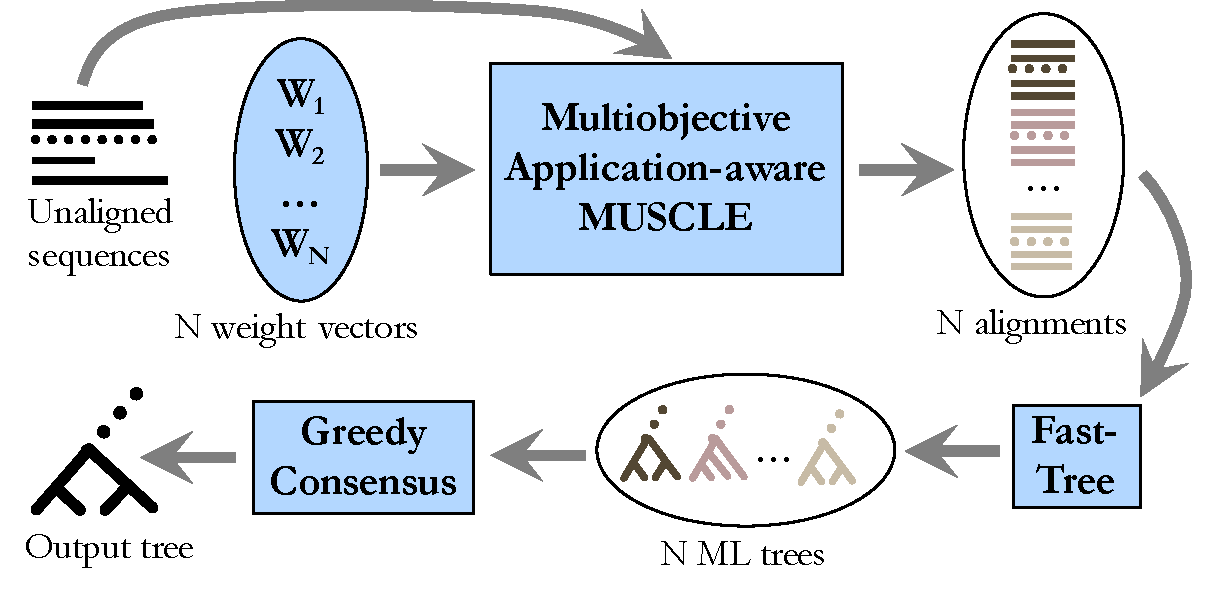
\includegraphics[width=0.9\textwidth]{Figure/workflow.pdf}
	\caption{Simplified pipeline of MAMMLE framework. The components marked with a blue shade can potentially be modified, replaced, or further refined by bioinformatics researchers and practitioners.}
	\label{fig:workflow}
\end{figure}
%\vspace{-12 mm}

\section{Methods}
The phylogenetic reconstruction pipeline of MAMMLE is illustrate in Figure~\ref{fig:workflow}. The components open to modification are marked with a blue shade. It starts by feeding the unaligned sequences to the system, which simultaneously optimizes four application-aware objectives with the help of $N$ well-distributed 4D weight vectors given as input and generate $N$ (in this article $N=30$) alternative alignments (please refer to Section~\ref{sec:ma-muscle} for details). %We choose to work with MUSCLE due to its simplicity and efficacy. %Although we use MUSCLE in this article due to its simplicity and efficacy, it can be replaced by other iterative MSA methods. 
Next, MAMMLE infers a ML tree from each of the $N$ alignments using FastTree (\cite{price2010fasttree}). We prefer FastTree over other ML methods due to its speed. Finally, MAMMLE summarizes the $N$ ML trees using a simple greedy consensus method of PAUP* (Phylogenetic Analysis Using PAUP) available at \url{https://paup.phylosolutions.com}. Any tree summarizing approach can be employed here. Note that MAMMLE relieves the user from parameter tuning through its well-spaced weight vectors and thus we used default parameter settings of MUSCLE and FastTree. The important components are further discussed in subsequent sections.

%\vspace{-4 mm}


\subsection{MO Application-aware MUSCLE} \label{sec:ma-muscle}

\subsubsection{Application-aware objective functions}
To design MO application-aware MUSCLE, we embed the four simple objective functions, identified in Chapter~\ref{ch:cybernatics} based on their better correlation to the tree accuracy, within the iterative refine phase of MUSCLE. Several pairs of these objectives may have conflicting relationship (please see Chapter~\ref{ch:cybernatics}). For the sake of ease, we repeat them as follows.
\begin{enumerate}
	\item Maximize similarity for columns containing gaps (SIMG): For each column of the MSA having at least one gap, it calculates the ratio of the most frequent characters. Then all those ratios are added to get the SIMG score.
	\item Maximize similarity for columns containing no gaps (SIMNG): This is similar to SIMG except that it considers those columns of the MSA that do not have any gap.
	\item Maximize sum-of-pairs (SP): For each pair of aligned sequences in the MSA, it takes the sum of substitution score for the two aligned characters across all columns using a substitution matrix. The addition of all pairwise scores gives the SOP score. In this chapter, we use the BLOSUM62 matrix for protein sequences.
	\item Minimize the number of gaps (GAP): The summation of the number of gap characters in each aligned sequence. For the sake of uniformity, we convert this score into a maximization criterion.
\end{enumerate}


\subsubsection{MO principles}
The goal of an multi-objective (MO) algorithm is to generate a set of solutions, popularly known as the Pareto-optimal solutions in the MO literature, which represent the best compromise among the (conflicting) objectives. 
%In the MO literature, these solutions are popularly said to constitute the Pareto front of the solution space. 
Among the several classes of MO algorithms (e.g., pareto-based, decomposition-based, indicator-based, etc.), decomposition-based strategies are found effective to face the difficulties in handling `many' (i.e., more than three) objectives~\cite{li2015many}. These algorithms decompose the task of generating several alternative solutions into many single-objective problems with the help of a set of well-distributed weight vectors, popularly known as reference directions. Each weight vector aggregates the different objective scores into a single value that eventually leads to one member of the final solution set.

\begin{figure}[!htbp]
	\centering
	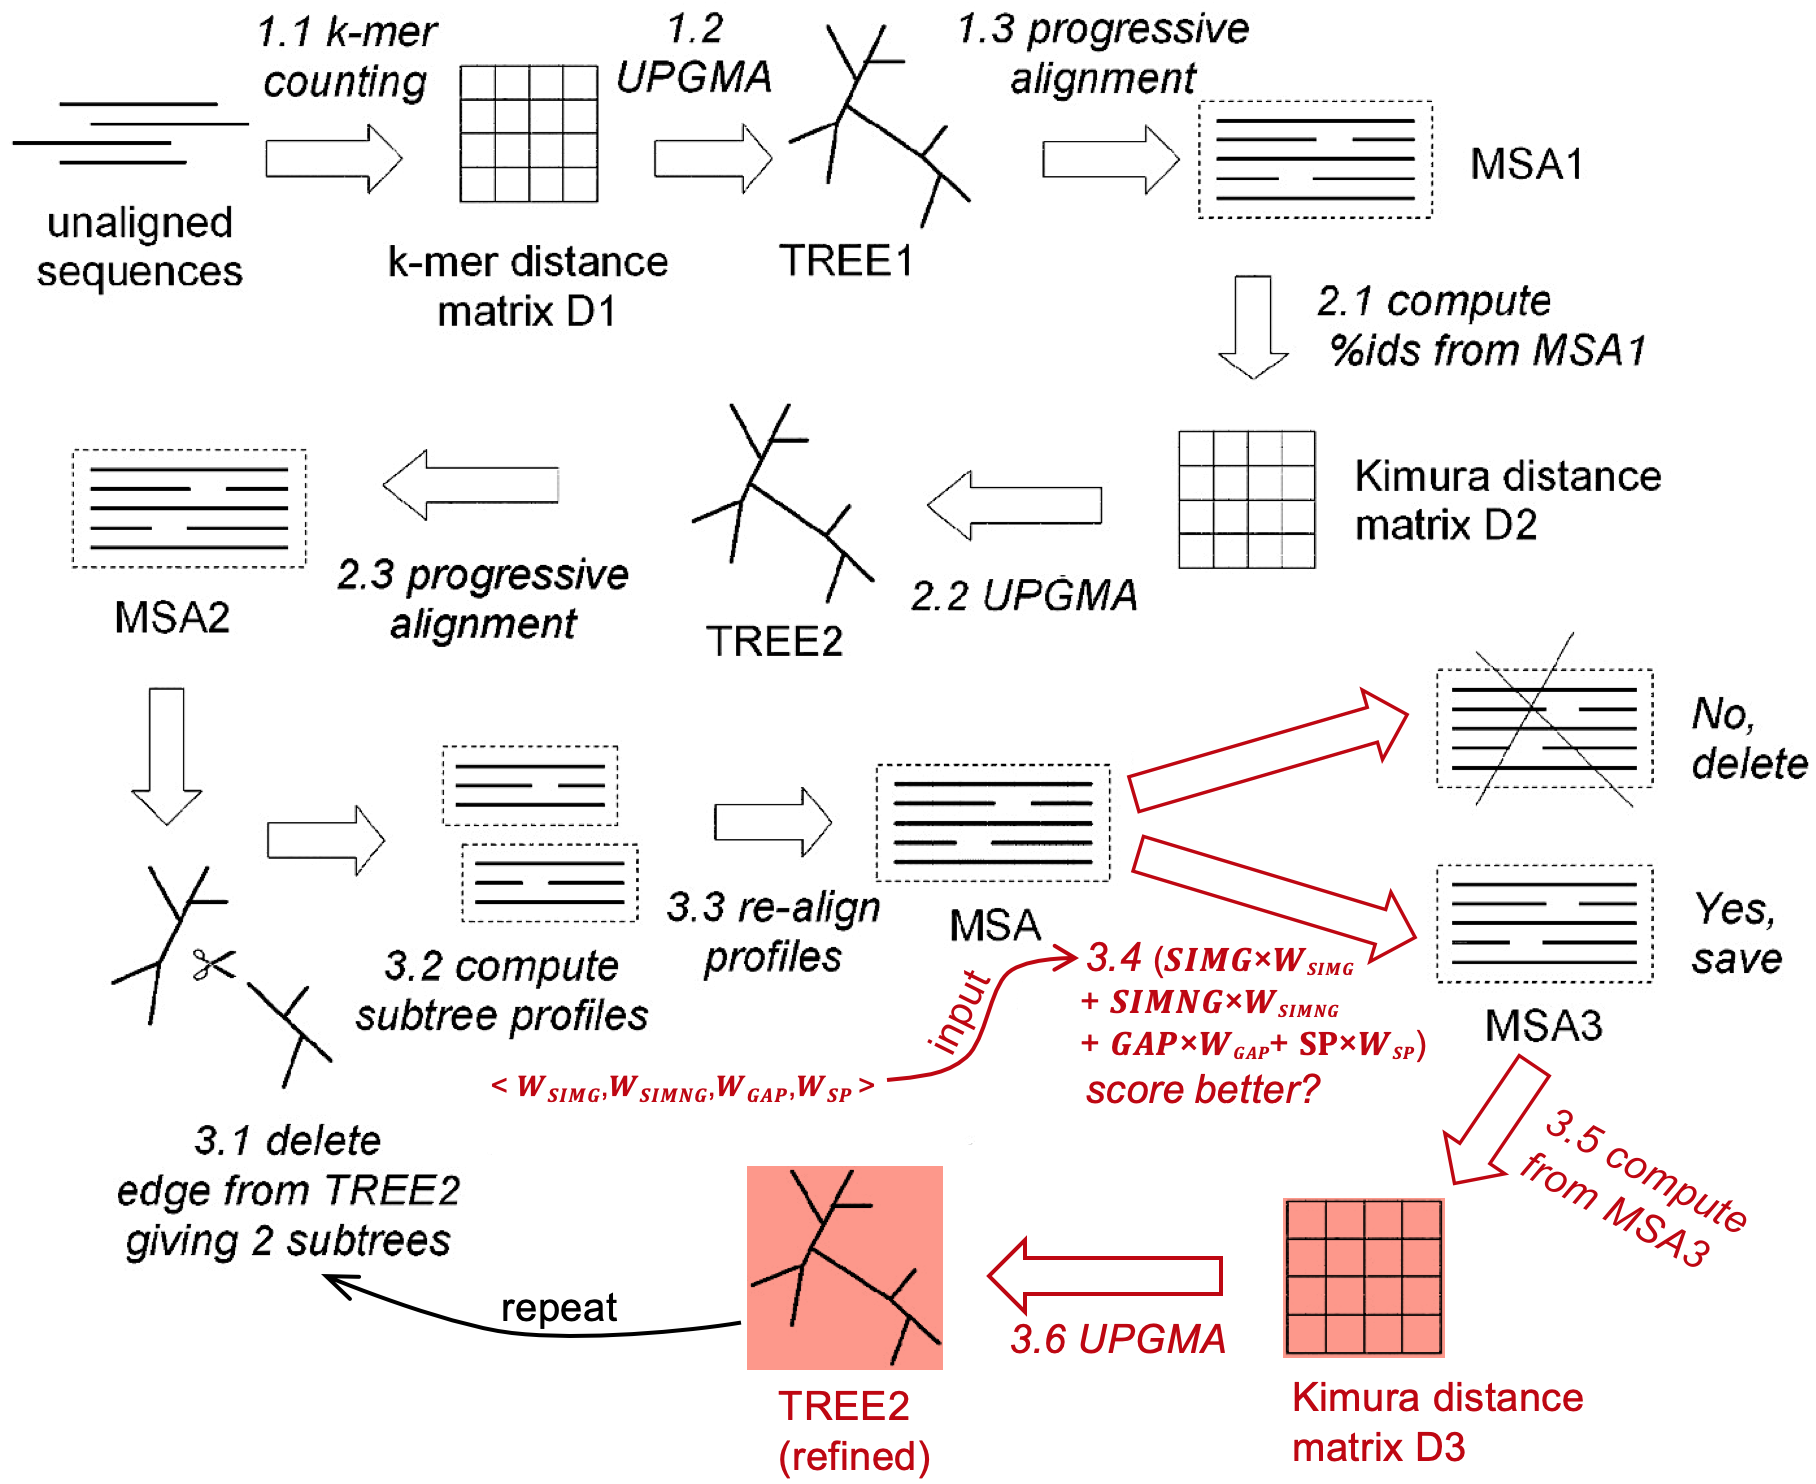
\includegraphics[width=0.9\textwidth]{Figure/ma-muscle}
	\caption{High-level workflow of MO application-aware MUSCLE for a single weight vector. Steps (3.4 to 3.6) added/modified on the original MUSCLE are marked with red color. This figure is modification of the original image taken from~\cite{edgar2004muscle}.}
	\label{fig:ma-muscle}
\end{figure}

\subsubsection{Simplified workflow}
We drive the iterative search process of MUSCLE with a total of four objectives directed by a 4D weight vector. Figure~\ref{fig:ma-muscle} depicts a high-level workflow for one weight vector, where the steps (3.4 to 3.6) inspired by the MO approach are marked as red. This workflow is executed for all weight vectors to get alternative solutions and can be performed independently in parallel. %As will be evident later, PMAO treats a solution better than the other based on the weighted-sum of four objective values instead of using ML score alone. 
Also note that, unlike original MUSCLE, we update the guide tree (step 3.6) each time a better MSA is obtained to intensify the effect of MO principles.

\subsubsection{Weight vectors}
Although working with a higher number of weight vectors increase the chance of getting better solutions in the solution set, we choose to work with 30 weight vectors to reduce the computational burden as well as to demonstrate the synergy between MUSCLE and an MO approach since 30 is quite a low number to tackle four objectives alone by an MO algorithm~\cite{deb2014evolutionary}. We calculate 30 well-spaced points on a 4D unit simplex using the method suggested by~\cite{ref_dirs_energy} as our weight vectors. Each of the 30 vertical bars in Figure~\ref{fig:30-weights} depicts one weight vector. %The workflow of


\begin{figure}[!htbp]%
	%\begin{adjustwidth}{-1.3cm}{}
	\centering
	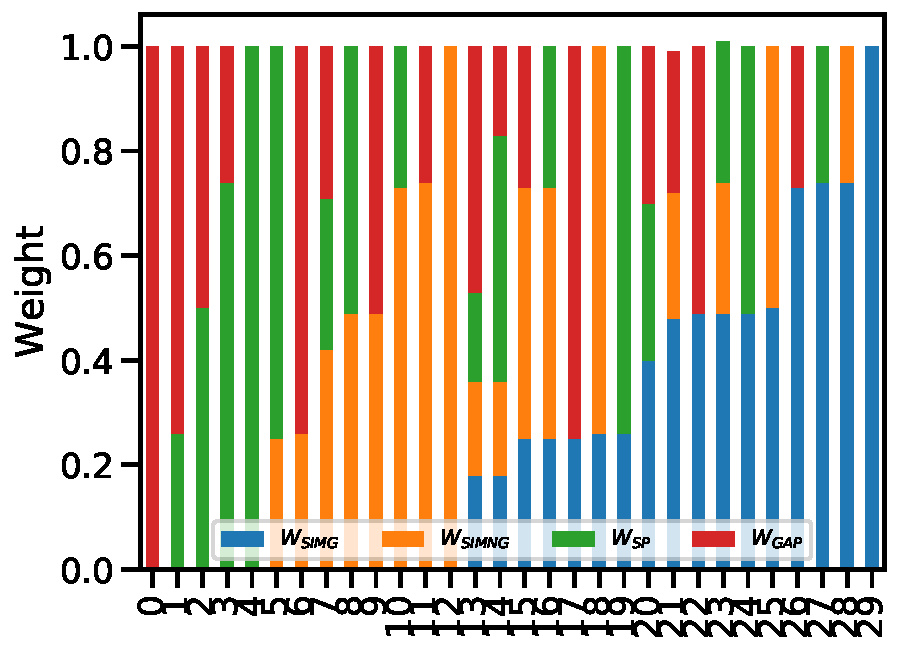
\includegraphics[width=0.6\textwidth]{Figure/30-4D-weight}
	\caption{30 well-spaced 4D weight vectors. Each vertical bar depicts one weight vector.}
	\label{fig:30-weights}
	%\end{adjustwidth}
\end{figure}

\subsection{Greedy Consensus}

Greedy consensus of a set of given trees is constructed by sequentially
adding one clade at a time, the most frequently occurring clade that is compatible with clades already included
in the greedy consensus tree breaking ties randomly if necessary.
This process
ends when the parietal being constructed is fully resolved which is also known as a bifurcating tree. 
Greedy consensus tree is also known ``majority rule extended''~\cite{phylip}, and  implemented in PAUP*~\cite{swofford_paup*_2002}. 

\subsection{Tree Accuracy Measure} 
We evaluate the accuracy of each estimated phylogenetic tree with respect to the reference phylogenetic tree using a widely used measure known as the False Negative (FN) rate. FN rate is the percentage of edges present in the true tree but missing in the estimated tree. So a small value of FN rate is desirable. Although there are two more common tree error measures (False Positive (FP rate) and and Robinson-Foulds (RF) rate), all of them are identical when true and estimated trees are binary~\citep{warnow2017computational}. In this thesis we worked with binary trees only. %as a quality measure, 

\subsection{Datasets}
We conduct our experiments on the BAliBASE 3.0 benchmark~\cite{thompson2005balibase} which is considered to be the de facto standard for biological alignment database of protein families. It provides manually refined reference alignments of high quality based on 3D structural superposition. It has 218 datasets which are organized into six groups according to their families and similarities: RV11 (very divergent sequences, residue identity below 20\%), RV12 (medium to divergent sequences, 20\%-40\% residue identity), RV20 (families with one or more highly divergent sequences), RV30 (divergent subfamilies), RV40 (sequences with large terminal N/C extensions), and RV50 (sequences with large internal insertions). 

As we adopt the FN rate as our domain-specific performance measure, following the strategy of~\cite{mirarab2015pasta} we generate a reference tree for each dataset by inferring an ML tree from the reference alignments using RAxML~\cite{stamatakis2014raxml} with bootstrap analysis and retaining only the highly supported edges.



\section{Results and discussion }
We compared MAMMLE with MUSCLE (with FastTree) on the most widely-used BAliBASE 3.0 benchmark (\cite{thompson2005balibase}) of protein families using the FN rate (percentage of true tree edges missing in the estimated tree) as the accuracy measure. Following the principles used by~\cite{mirarab2015pasta}, we avoid the instances with a lower number (i.e., below 11) of sequences. % and generate a reference tree for 147 considered instances by RAxML (\cite{stamatakis2014raxml}) bootstrap analysis on the reference alignment.

%\section{Dataset} 
% Table generated by Excel2LaTeX from sheet 'mammle'
\begin{table}[htbp]
	\centering
	\caption{Dividing 147 BAliBASE 3.0 instances into 7 size levels based on number of sequences and average sequence length.}
	\begin{tabular}{r|r|r}
		\multicolumn{1}{l|}{Instance size} & \multicolumn{1}{l|}{Max. (no. of seq. $\times$ avg. seq. len.)} & No. of instances\\
		\hline
		1     & 5040.9997 & 20 \\
		\hline
		2     & 6955.0004 & 22 \\
		\hline
		3     & 9816.0012 & 22 \\
		\hline
		4     & 12915 & 22 \\
		\hline
		5     & 19598.0013 & 20 \\
		\hline
		6     & 32777 & 20 \\
		\hline
		7     & 57848.9966 & 21\\
		\hline
	\end{tabular}%
	\label{tab:data-size}%
\end{table}%

%\subsection{Best Accuracy from MO Application-ware MUSCLE}

\begin{figure}[!htbp]%
	\begin{adjustwidth}{-1.2cm}{}
		\centering
		\begin{subfigure}{0.40\textwidth} 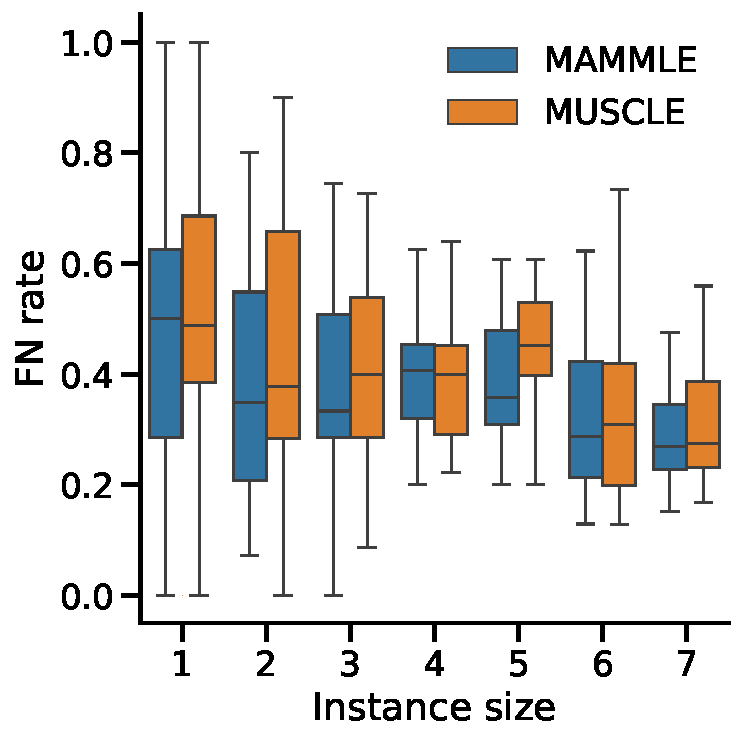
\includegraphics[width=\textwidth]{Figure/comparison} \caption{FN rate distribution} \label{fig:boxplot} \end{subfigure}
		\begin{subfigure}{0.40\textwidth} 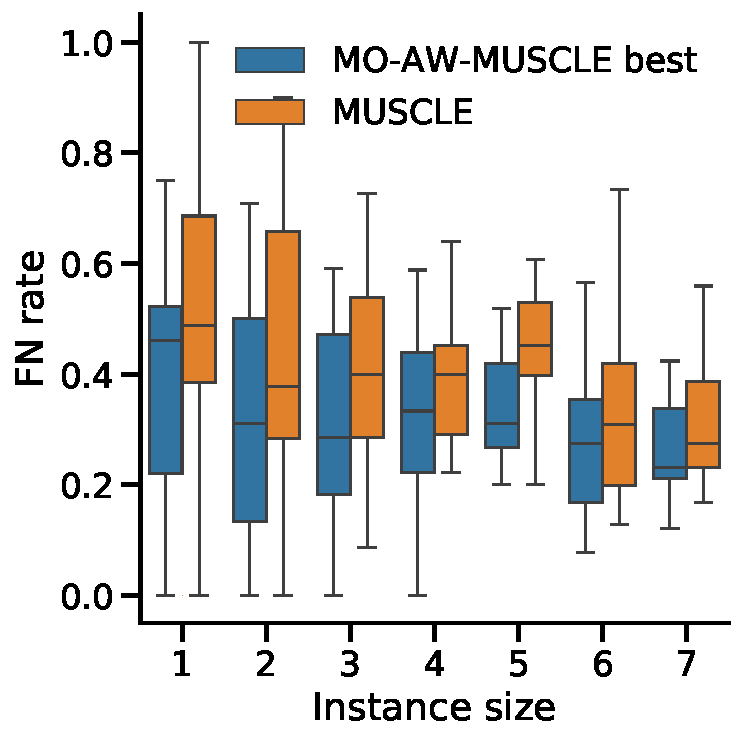
\includegraphics[width=\textwidth]{Figure/comparison-momuscle} 
			%\caption{FN rate distribution} \label{fig:boxplot} 
		\end{subfigure}
		\begin{subfigure}{0.40\textwidth} 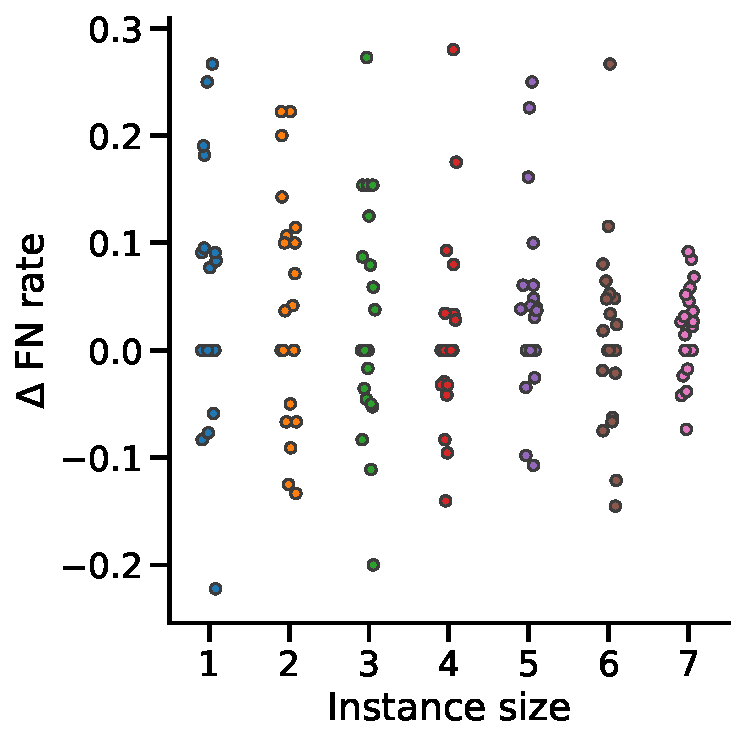
\includegraphics[width=\textwidth]{Figure/delta3} \caption{ FN rate improvement}\label{fig:scatter}\end{subfigure}
		\begin{subfigure}{0.40\textwidth} 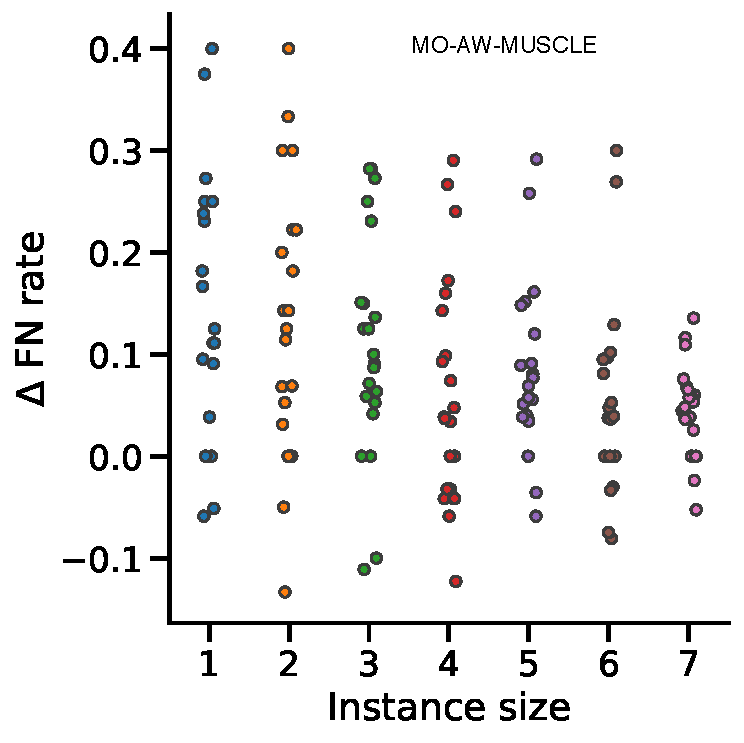
\includegraphics[width=\textwidth]{Figure/delta4-momuscle} 
			%\caption{MAMMLE: FN rate improvement}\label{fig:scatter}
		\end{subfigure}
		
		\begin{subfigure}{0.40\textwidth} 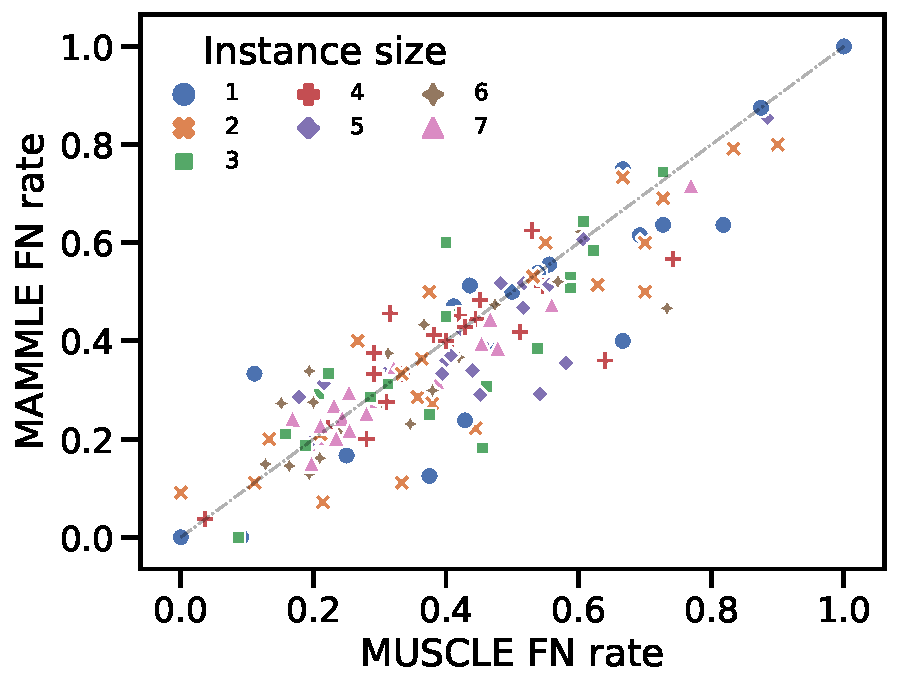
\includegraphics[width=\textwidth]{Figure/delta5} \caption{Individual FN rate}\label{fig:scatter_fn}\end{subfigure}
		\begin{subfigure}{0.40\textwidth} 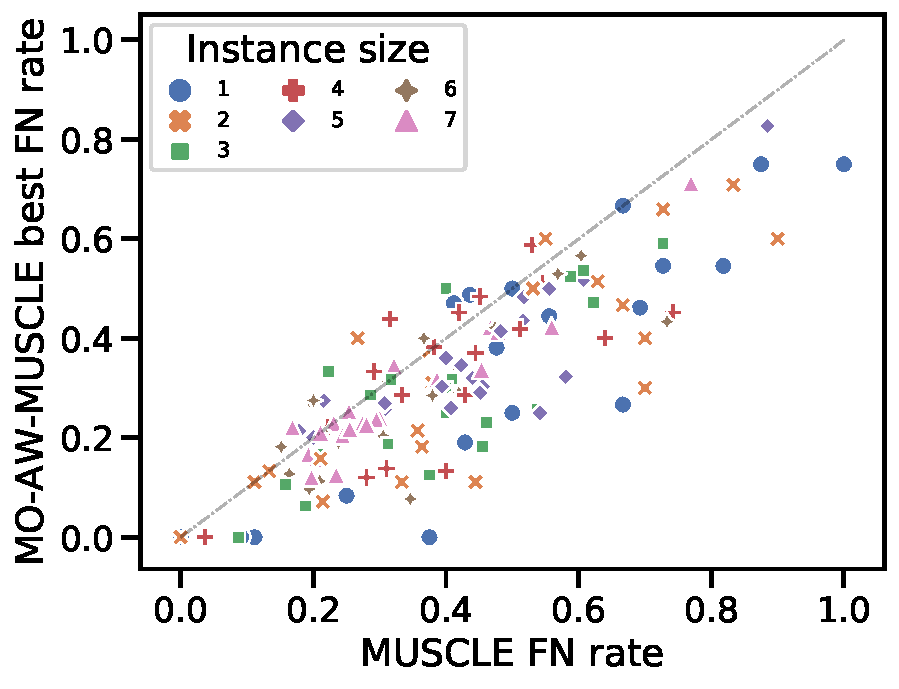
\includegraphics[width=\textwidth]{Figure/delta5-momuscle} 
		%	\caption{Individual FN rate: MUSCLE vs MAMMLE}\label{fig:scatter_fn}
		\end{subfigure}
	\end{adjustwidth}
	\caption[Close examination of MAMMLE (MO-AW-MUSCLE) vs MUSCLE]{Close examination of MAMMLE (MO-AW-MUSCLE) vs MUSCLE. Top panel (i.e., part (a)) shows the FN rate distribution of MAMMLE (MO-AW-MUSCLE) vs MUSCLE. Middle panel (i.e., part (b))) shows the FN rate improvement of MAMMLE (MO-AW-MUSCLE) over MUSCLE. Bottom panel (i.e., part (c)) shows the individual FN rate of MAMMLE (MO-AW-MUSCLE) against that of MUSCLE for each instance. The left (right) column represents results for MAMMLE (MO-AW-MUSCLE) }
	\label{fig:mammle-result}
\end{figure}



%\subsection{Performance of MAMMLE }

%\begin{figure}[!htbp]%
%	\begin{adjustwidth}{-1.1cm}{}
%		\centering
%		\begin{subfigure}{0.50\textwidth} 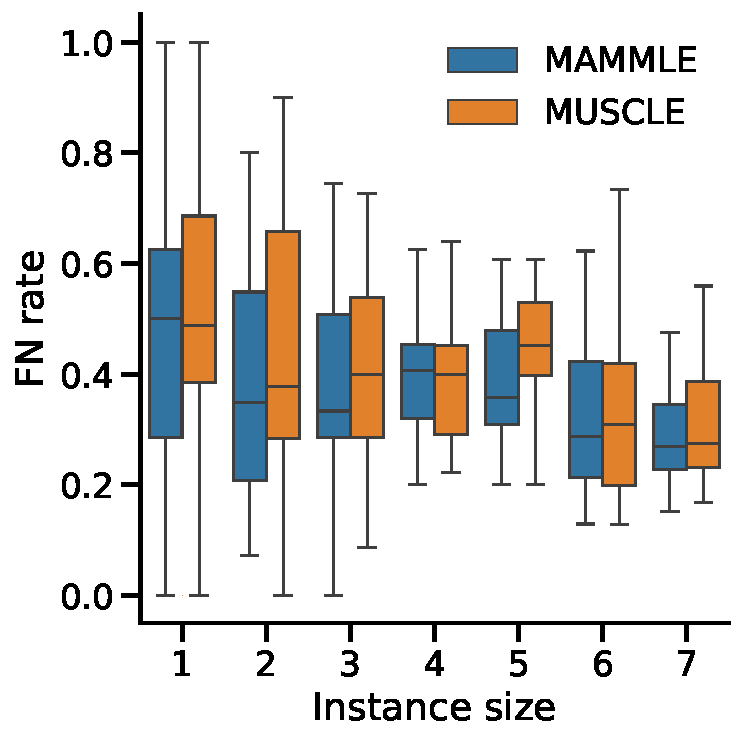
\includegraphics[width=\textwidth]{Figure/comparison} \caption{FN rate distribution} \label{fig:boxplot} \end{subfigure}
%		\begin{subfigure}{0.50\textwidth} 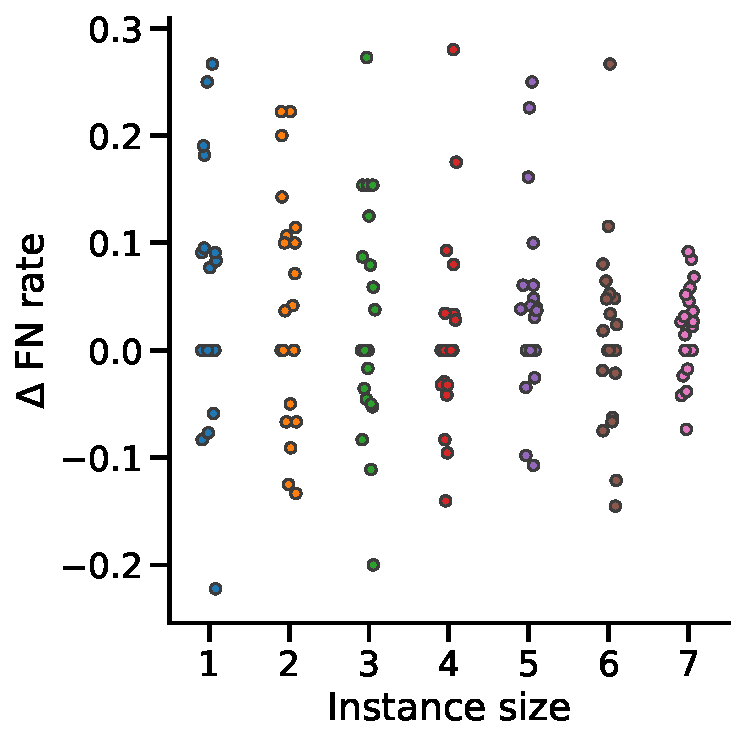
\includegraphics[width=\textwidth]{Figure/delta3} \caption{MAMMLE: FN rate improvement}\label{fig:scatter}\end{subfigure}
%		\begin{subfigure}{0.60\textwidth} 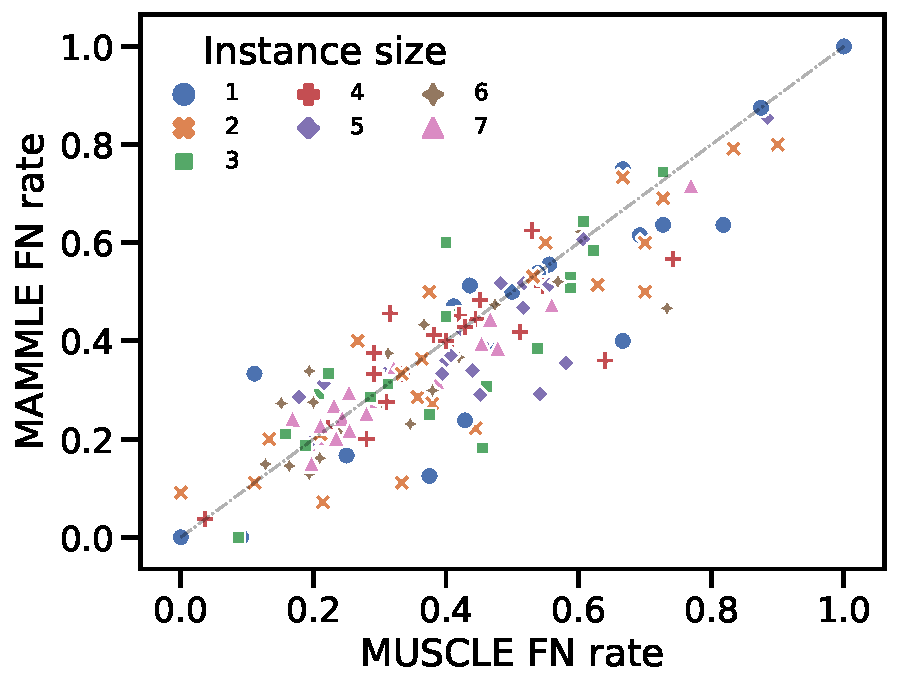
\includegraphics[width=\textwidth]{Figure/delta5} \caption{Individual FN rate: MUSCLE vs MAMMLE}\label{fig:scatter_fn}\end{subfigure}
%	\end{adjustwidth}
%	\caption{Close examination of MAMMLE vs MUSCLE.}
%	\label{fig:mammle-result}
%\end{figure}

Among the 147 instances, MAMMLE performs better in 74 cases and worse in 43 cases than MUSCLE (supplementary Table~\ref{tab:muscle-mammle-all} in Appendix~\ref{apendix:mammle}). We conduct the \textit{one-sided} (i.e., null hypothesis: median FN rate of MUSCLE is better than MAMMLE) Wilcoxon signed ranks test at 95\% confidence level where the null hypothesis is rejected with $p$-value=0.001. To get more insight, we divide the 147 instances into 7 levels of instance size, considering their number of sequences and average sequence length as shown in Table~\ref{tab:data-size}, each level having 20-22 instances. We examine the performance of MAMMLE with respect to MUSCLE in the left column of Figure~\ref{fig:mammle-result}. We also show the comparative results of the best FN rate from MO application-aware MUSCLE (MO-AW-MUSCLE) against MUSCLE in the right column of Figure~\ref{fig:mammle-result}, to demonstrate the potential of MO strategy and usefulness of the ensemble approach of MAMMLE. We see that the best FN rate achieved by MO-AW-MUSCLE is clearly better than that of MUSCLE except for a few instances.
Figure~\ref{fig:boxplot} depicts the FN rate distribution of MAMMLE and MUSCLE across different instance sizes. We see that MAMMLE helps to get better accuracy in all levels except 4 and 6. Notably, variance of both MAMMLE and MUSCLE reduces as the instance size increases; this can be attributed to the fact that ML approach performs better as the data size increases. 

To complement Figure~\ref{fig:boxplot}, we visualize the improvement achieved by MAMMLE by plotting the individual FN rates and MUSCLE FN rate $-$ MAMMLE FN rate for the instances of each level in Figure~\ref{fig:scatter_fn} (scatterplot) and Figure~\ref{fig:scatter} (\textit{stripplot}; adjusts the position of points having similar FN rate for the ease of perception) respectively. Points below (above) the diagonal line (horizontal line at $\Delta$FN rate=0) in Figure~\ref{fig:scatter_fn} (Figure~\ref{fig:scatter}) represent the instances where MAMMLE outperforms MUSCLE. Evidently, the maximum improvement registered by MAMMLE is around 27\% across different levels (Figure~\ref{fig:scatter}). Figure~\ref{fig:scatter_fn} offers further insights. MUSCLE performed worse mostly for the smaller instances (Levels 1-4), which are presumed to be difficult for the ML approach; and here MAMMLE outperforms MUSCLE. On the other hand, MUSCLE outperforms MAMMLE mostly for the larger instances where ML approach performs well anyway. Also, observe that MAMMLE outperforms MUSCLE mostly in the cases when MUSCLE FN rate $> 0.6$. 
%The instances where (MUSCLE FN rate $> 0.6$) are mostly of smaller levels (1-4) (i.e., difficult for the ML approach) and in those cases MAMMLE outperforms MUSCLE. 
%On the other hand, MUSCLE outperforms MAMMLE mostly on the cases where (MUSCLE FN rate $< 0.6$) and dominated by the larger instances. 

In summary, although, MAMMLE's improved cases are distributed across all levels and a wider range of FN rates, the improvement seems higher on the smaller instances, indicating that MAMMLE possesses the potential to yield better trees with limited data (e.g., to estimate gene tree on fewer/smaller gene sequences which is challenging for ML approach). 
However, the cases (45 out of 147) where MUSCLE is better (within 15\%) demands further research effort to enhance the current ensemble method (i.e., greedy consensus).

%Although, MAMMLE's improved cases are distributed across all size levels and a wider range of FN rate, the improvement seems higher on the smaller instances. All these indicate to a potential strength of MAMMLE to yield better trees with limited data (e.g., to estimate gene tree on fewer/smaller gene sequences challenging for ML approach). 
%However, the cases (45 out of 147) where MUSCLE is better (within 15\%) ask more research effort to enhance the current ensemble method (i.e., greedy consensus). 

\subsection{MAMMLE with Ensemble based on Quartet Consistency}
Now we analyze the performance of MAMMLE by using a different ensemble approach which is summarizing the generated ML trees based on quartet consistency score using ASTRAL~\cite{zhang2018astral}, one of the most accurate and widely used coalescent-based methods to infer species trees. Please recall that, the quartet score of a candidate summarized tree $T$ is the total, across all the input trees, of the number of induced quartet trees that $T$ agrees with. We examine the performance of MAMMLE with respect to MUSCLE in the left column of Figure~\ref{fig:mammle-result-ast}. We also show the comparative results of the best FN rate from MO application-aware MUSCLE (MO-AW-MUSCLE) against MUSCLE in the right column of Figure~\ref{fig:mammle-result-ast}.

Among the 147 instances, MAMMLE performs better in 68 cases and worse in 41 cases than MUSCLE (supplementary Table~\ref{tab:muscle-mammle-all} in Appendix~\ref{apendix:mammle}). We conduct the \textit{one-sided} (i.e., null hypothesis: median FN rate of MUSCLE is better than MAMMLE) Wilcoxon signed ranks test at 95\% confidence level where the null hypothesis is rejected with $p$-value=0.001. 
Figure~\ref{fig:boxplot-ast} depicts the FN rate distribution of MAMMLE and MUSCLE across different instance sizes. 
To complement Figure~\ref{fig:boxplot-ast}, we visualize the improvement achieved by MAMMLE by plotting the individual FN rates and MUSCLE FN rate $-$ MAMMLE FN rate for the instances of each level in Figure~\ref{fig:scatter-fn-ast} (scatterplot) and Figure~\ref{fig:scatter-ast} (stripplot) respectively. Points below (above) the diagonal line (horizontal line at $\Delta$FN rate=0) in Figure~\ref{fig:scatter-fn-ast} (Figure~\ref{fig:scatter-ast}) represent the instances where MAMMLE outperforms MUSCLE. The maximum improvement registered by MAMMLE is around 35\% across different levels (Figure~\ref{fig:scatter-ast})
From all these results, it seems that the MAMMLE with ASTRAL based ensemble is not better than that of the simple greedy consensus based ensemble. 

\begin{figure}[!htbp]%
	\begin{adjustwidth}{-1.2cm}{}
		\centering
		\begin{subfigure}{0.40\textwidth} 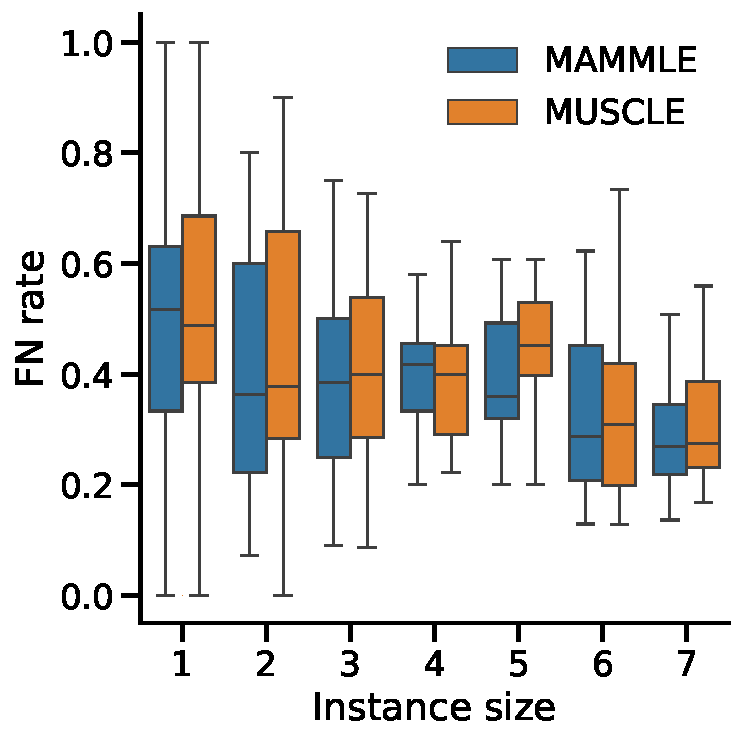
\includegraphics[width=\textwidth]{Figure/comparison-ast} \caption{FN rate distribution} \label{fig:boxplot-ast} \end{subfigure}
		\begin{subfigure}{0.40\textwidth} 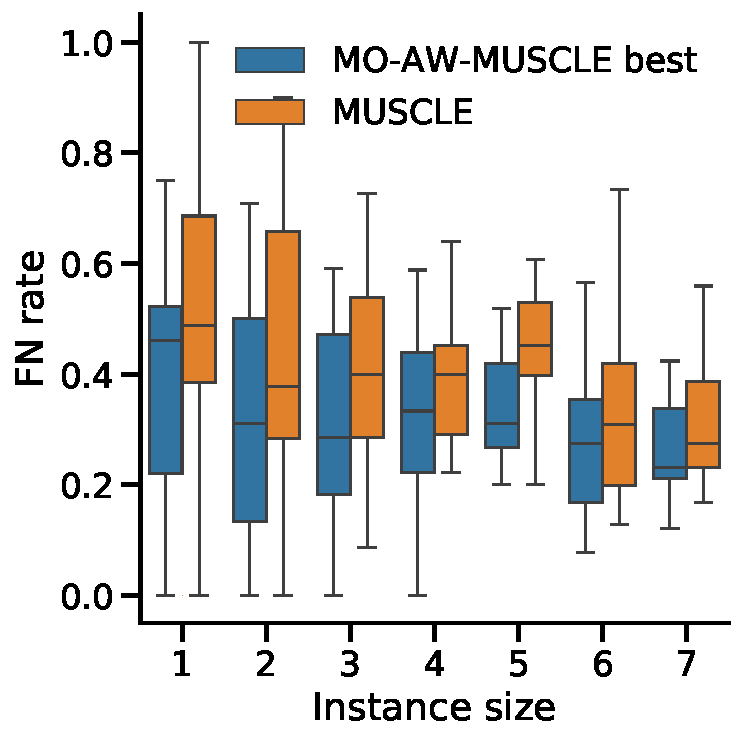
\includegraphics[width=\textwidth]{Figure/comparison-momuscle} 
			%\caption{FN rate distribution} \label{fig:boxplot} 
		\end{subfigure}
		\begin{subfigure}{0.40\textwidth} 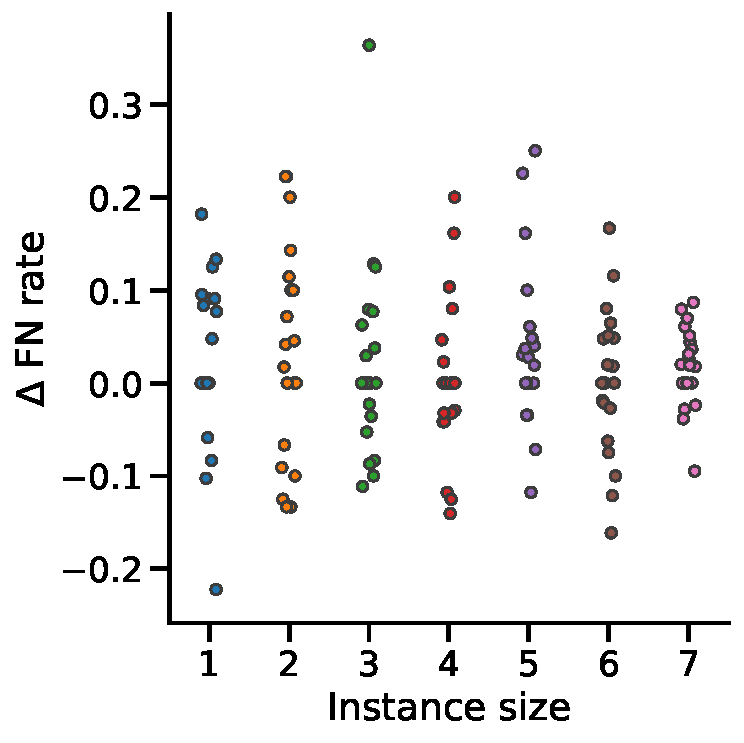
\includegraphics[width=\textwidth]{Figure/delta4-ast} \caption{ FN rate improvement}\label{fig:scatter-ast}\end{subfigure}
		\begin{subfigure}{0.40\textwidth} 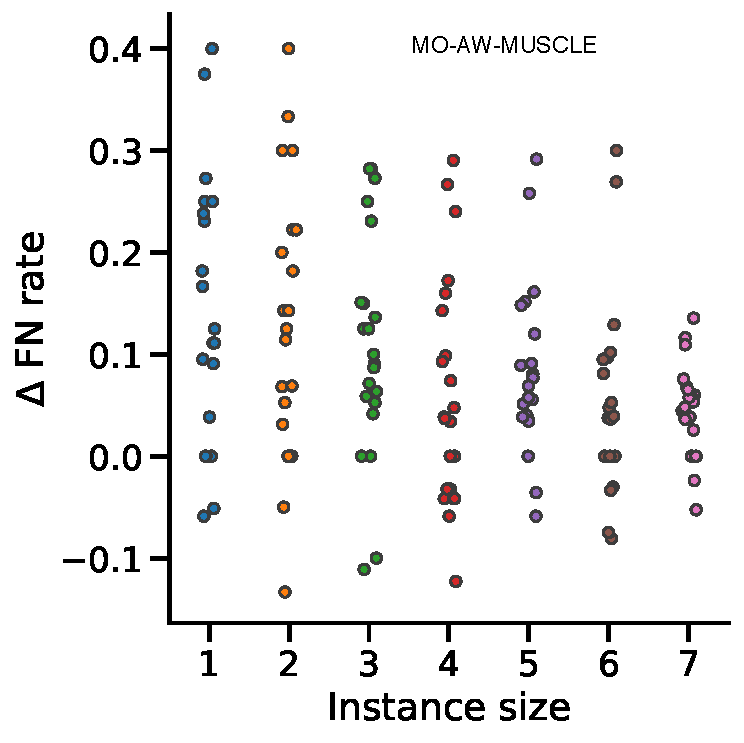
\includegraphics[width=\textwidth]{Figure/delta4-momuscle} 
			%\caption{MAMMLE: FN rate improvement}\label{fig:scatter}
		\end{subfigure}
		
		\begin{subfigure}{0.40\textwidth} 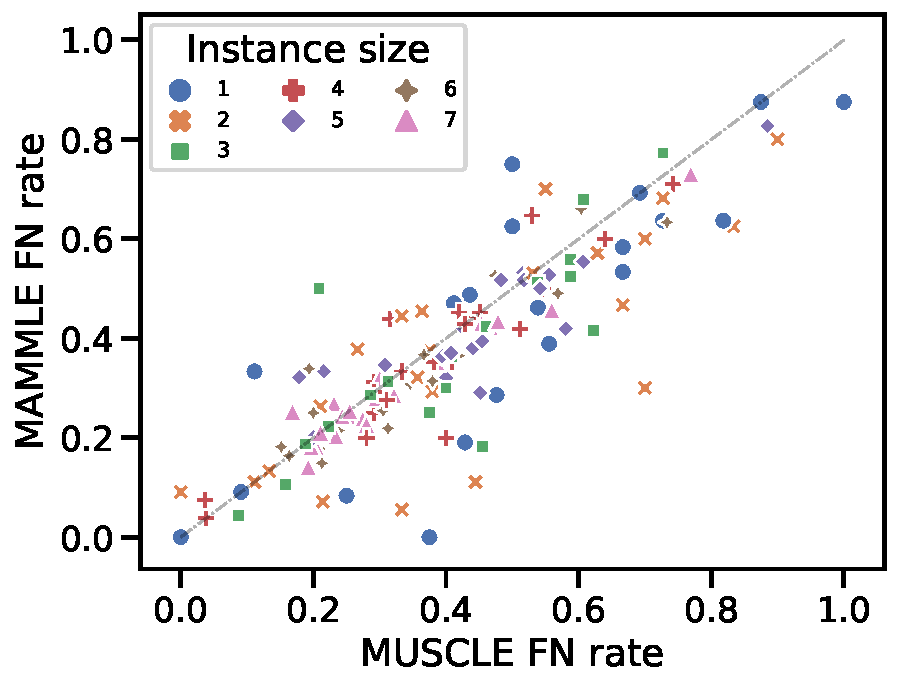
\includegraphics[width=\textwidth]{Figure/delta5-ast} \caption{Individual FN rate}\label{fig:scatter-fn-ast}\end{subfigure}
		\begin{subfigure}{0.40\textwidth} 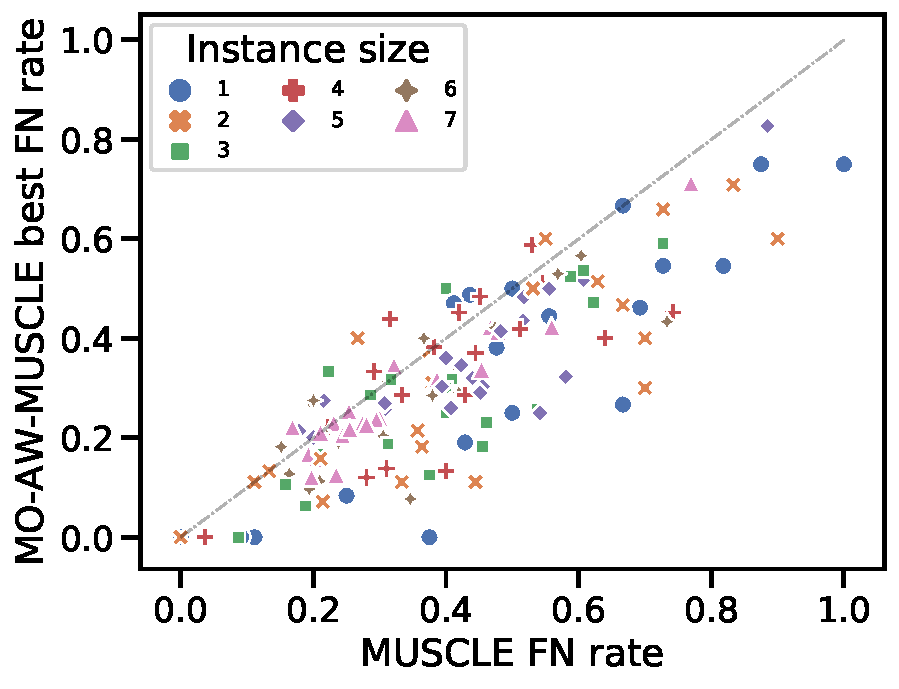
\includegraphics[width=\textwidth]{Figure/delta5-momuscle} 
			%	\caption{Individual FN rate: MUSCLE vs MAMMLE}\label{fig:scatter_fn}
		\end{subfigure}
	\end{adjustwidth}
	\caption[Close examination of MAMMLE with ASTRAL based ensemble (MO-AW-MUSCLE) vs MUSCLE]{Close examination of MAMMLE with ASTRAL based ensemble (MO-AW-MUSCLE) vs MUSCLE. Top panel (i.e., part (a)) shows the FN rate distribution of MAMMLE (MO-AW-MUSCLE) vs MUSCLE. Middle panel (i.e., part (b))) shows the FN rate improvement of MAMMLE (MO-AW-MUSCLE) over MUSCLE. Bottom panel (i.e., part (c)) shows the individual FN rate of MAMMLE (MO-AW-MUSCLE) against that of MUSCLE for each instance. The left (right) column represents results for MAMMLE (MO-AW-MUSCLE).}
	\label{fig:mammle-result-ast}
\end{figure}

%\begin{figure}[!htbp]%
%	\begin{adjustwidth}{-1.1cm}{}
%		\centering
%		\begin{subfigure}{0.50\textwidth} 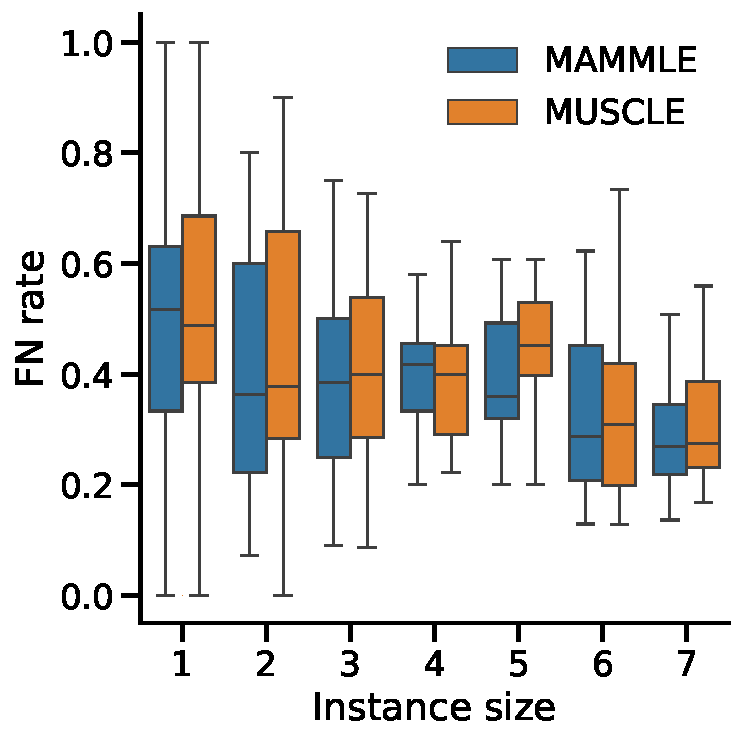
\includegraphics[width=\textwidth]{Figure/comparison-ast} \caption{FN rate distribution} \label{fig:boxplot-ast} \end{subfigure}
%		\begin{subfigure}{0.50\textwidth} 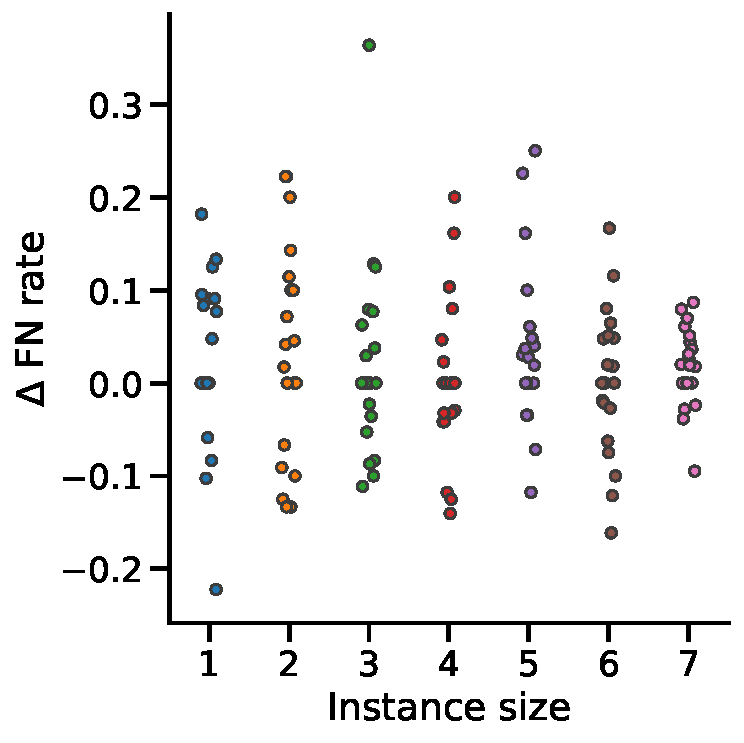
\includegraphics[width=\textwidth]{Figure/delta4-ast} \caption{MAMMLE: FN rate improvement}\label{fig:scatter-ast}\end{subfigure}
%		\begin{subfigure}{0.60\textwidth} 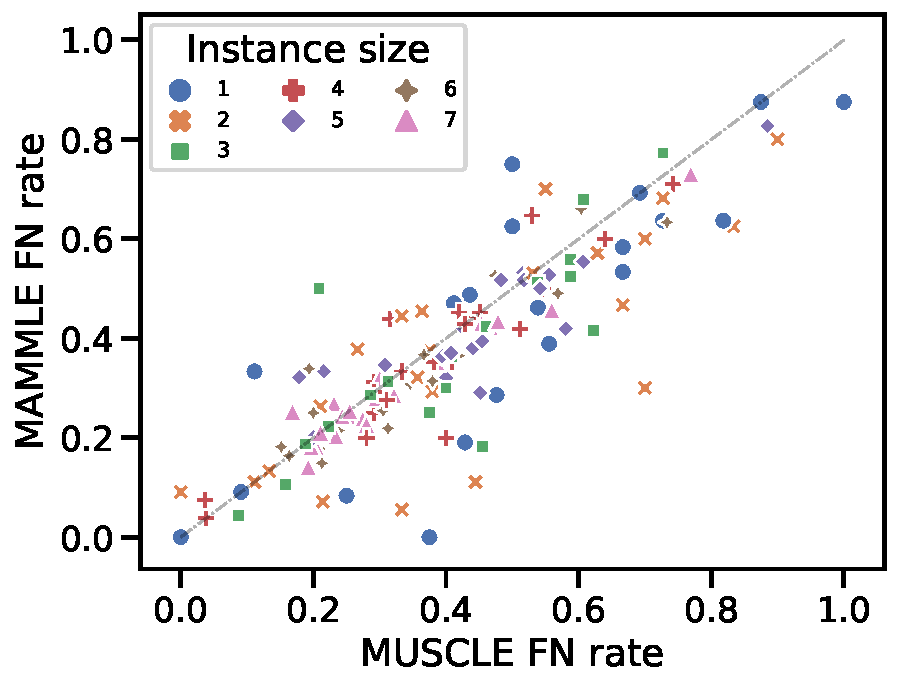
\includegraphics[width=\textwidth]{Figure/delta5-ast} \caption{Individual FN rate: MUSCLE vs MAMMLE}\label{fig:scatter-fn-ast}\end{subfigure}
%	\end{adjustwidth}
%	\caption{Close examination of MAMMLE vs MUSCLE.}
%	\label{fig:mammle-result-ast}
%\end{figure}

\subsection{Ensemble based on ML score from Concatenated MSAs}
Finally, we would like to access MAMMLE by using another ensemble method based on ML score from concatenated MSAs. Here, at first we concatenate the unique MSAs generated by MO-AW-MUSCLE to get a single average MSA. This concatenation helps to simultaneously consider all the phylogenetic signals contained in columns of the alternative MSAs generated by the MO approach as suggested by~\cite{ashkenazy2018multiple}.
Then we calculate ML score of the (average MSA, ML tree) pairs for each ML tree obtained from MO-AW-MUSCLE and select the pair with the highest tree as the output. We examine the performance of MAMMLE with respect to MUSCLE in the left column of Figure~\ref{fig:mammle-result-ast}. We also show the comparative results of the best FN rate from MO application-aware MUSCLE (MO-AW-MUSCLE) against MUSCLE in the right column of Figure~\ref{fig:mammle-result-ast}.

Among the 147 instances, MAMMLE performs better in 82 cases and worse in 37 cases than MUSCLE (supplementary Table~\ref{tab:muscle-mammle-all} in Appendix~\ref{apendix:mammle}). We conduct the \textit{one-sided} (i.e., null hypothesis: median FN rate of MUSCLE is better than MAMMLE) Wilcoxon signed ranks test at 95\% confidence level where the null hypothesis is rejected with $p$-value=$1.53\times10^{-5}$. 
Figure~\ref{fig:boxplot-ml} depicts the FN rate distribution of MAMMLE and MUSCLE across different instance sizes. 
To complement Figure~\ref{fig:boxplot-ml}, we visualize the improvement achieved by MAMMLE by plotting the individual FN rates and MUSCLE FN rate $-$ MAMMLE FN rate for the instances of each level in Figure~\ref{fig:scatter-fn-ml} (scatterplot) and Figure~\ref{fig:scatter-ml} (stripplot) respectively. Points below (above) the diagonal line (horizontal line at $\Delta$FN rate=0) in Figure~\ref{fig:scatter-fn-ml} (Figure~\ref{fig:scatter-ml}) represent the instances where MAMMLE outperforms MUSCLE. The maximum improvement registered by MAMMLE is around 40\% across different levels (Figure~\ref{fig:scatter-ml})
From all these results, we find that the MAMMLE variant with ML score based ensemble is the clearly ahead of the other two variants. However, this variant takes considerably larger time than the others.
\begin{figure}[!htbp]%
	\begin{adjustwidth}{-1.2cm}{}
		\centering
		\begin{subfigure}{0.40\textwidth} 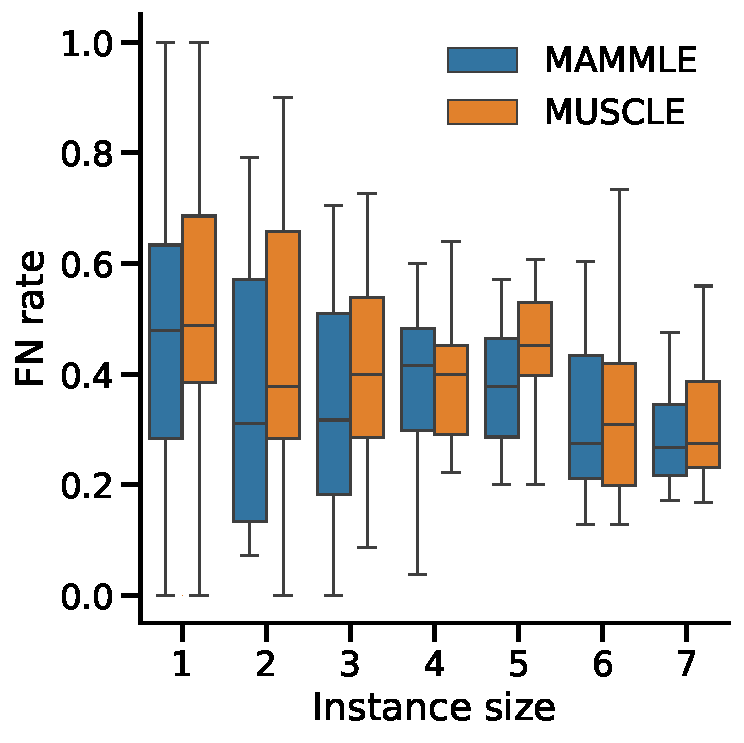
\includegraphics[width=\textwidth]{Figure/comparison-ml} \caption{FN rate distribution} \label{fig:boxplot-ml} \end{subfigure}
		\begin{subfigure}{0.40\textwidth} 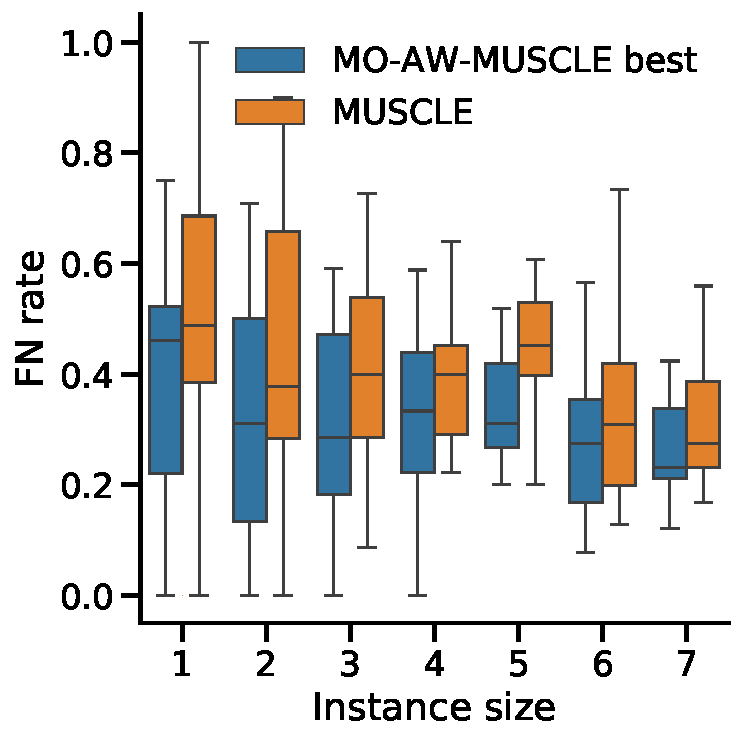
\includegraphics[width=\textwidth]{Figure/comparison-momuscle} 
			%\caption{FN rate distribution} \label{fig:boxplot} 
		\end{subfigure}
		\begin{subfigure}{0.40\textwidth} 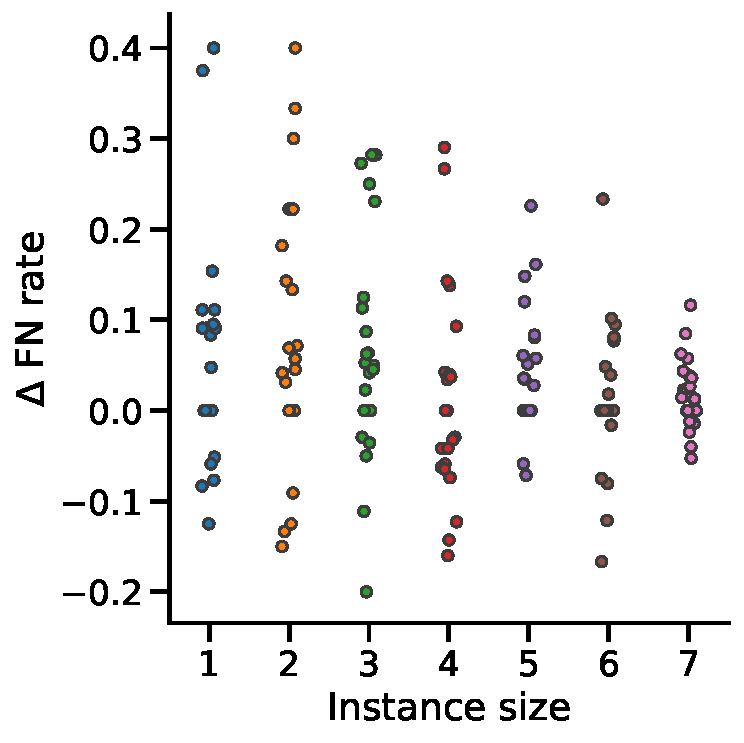
\includegraphics[width=\textwidth]{Figure/delta4-ml} \caption{ FN rate improvement}\label{fig:scatter-ml}\end{subfigure}
		\begin{subfigure}{0.40\textwidth} 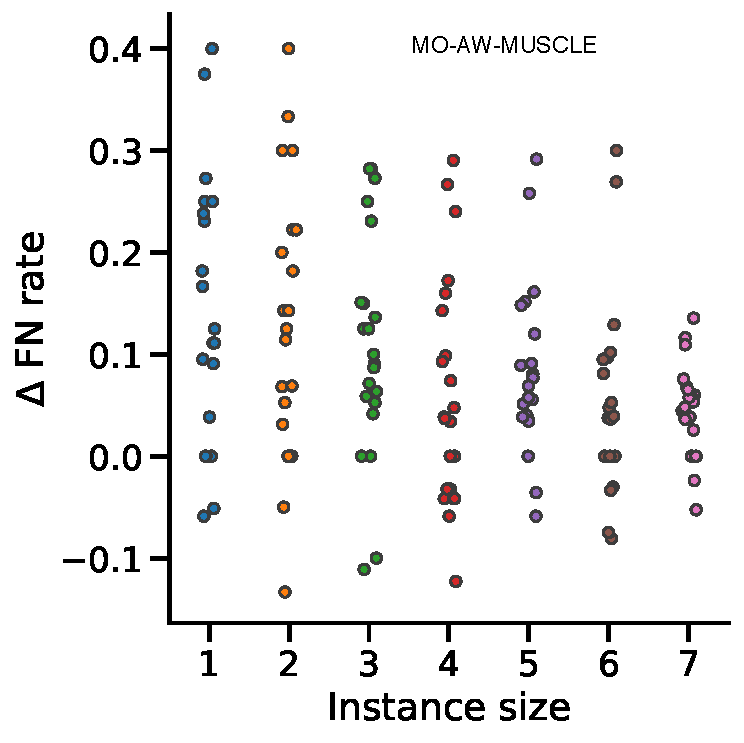
\includegraphics[width=\textwidth]{Figure/delta4-momuscle} 
			%\caption{MAMMLE: FN rate improvement}\label{fig:scatter}
		\end{subfigure}
		
		\begin{subfigure}{0.40\textwidth} 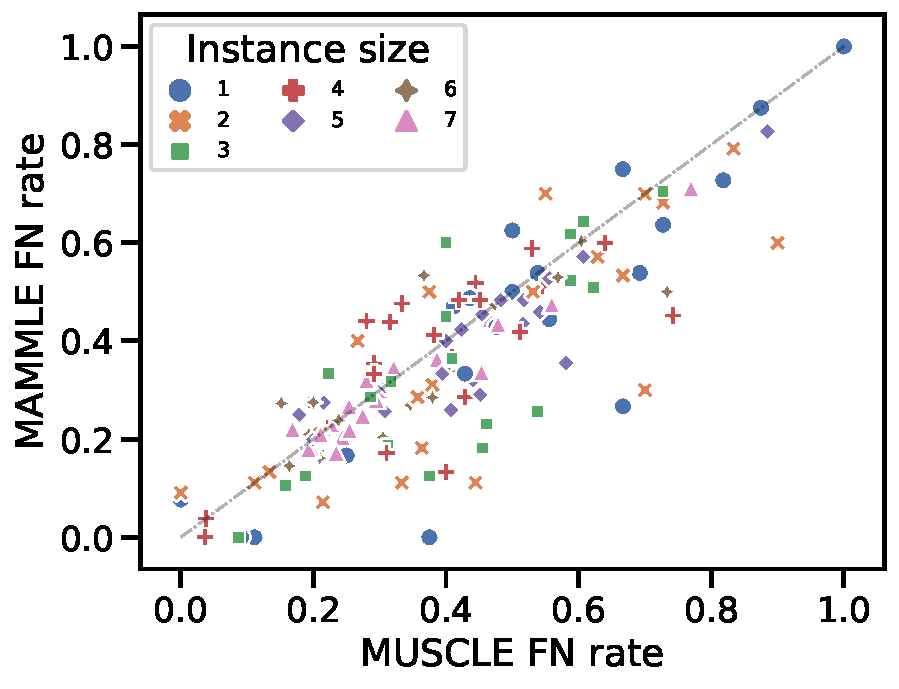
\includegraphics[width=\textwidth]{Figure/delta5-ml} \caption{Individual FN rate}\label{fig:scatter-fn-ml}\end{subfigure}
		\begin{subfigure}{0.40\textwidth} 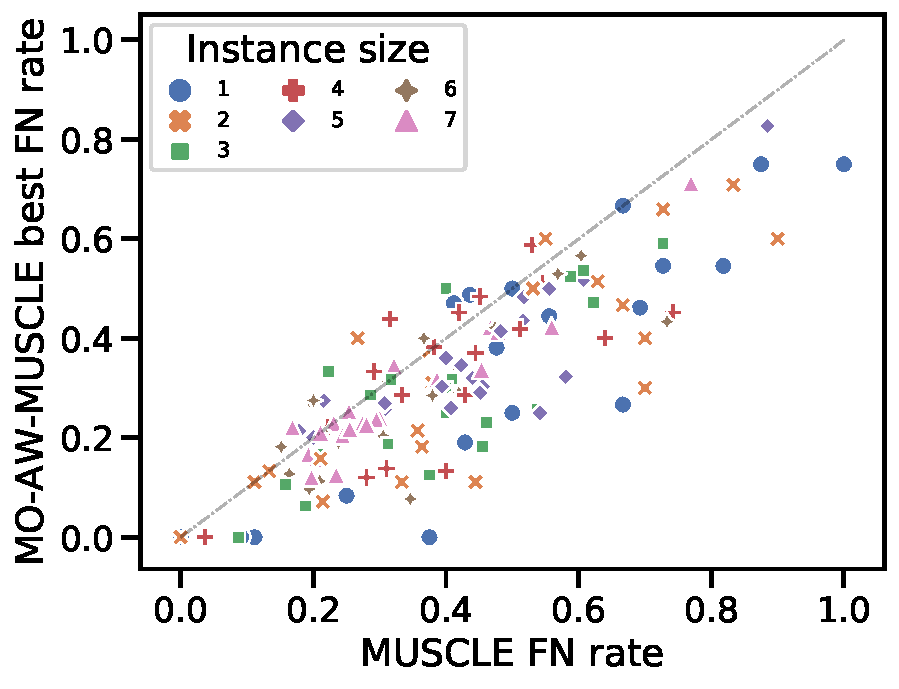
\includegraphics[width=\textwidth]{Figure/delta5-momuscle} 
			%	\caption{Individual FN rate: MUSCLE vs MAMMLE}\label{fig:scatter_fn}
		\end{subfigure}
	\end{adjustwidth}
	\caption[Close examination of MAMMLE with ML score based ensemble (MO-AW-MUSCLE) vs MUSCLE]{Close examination of MAMMLE with ML score based ensemble (MO-AW-MUSCLE) vs MUSCLE. Top panel (i.e., part (a)) shows the FN rate distribution of MAMMLE (MO-AW-MUSCLE) vs MUSCLE. Middle panel (i.e., part (b))) shows the FN rate improvement of MAMMLE (MO-AW-MUSCLE) over MUSCLE. Bottom panel (i.e., part (c)) shows the individual FN rate of MAMMLE (MO-AW-MUSCLE) against that of MUSCLE for each instance. The left (right) column represents results for MAMMLE (MO-AW-MUSCLE).}
	\label{fig:mammle-result-ml}
\end{figure}

\section{Conclusion}
In this chapter, we presented the MAMMLE framework which offers an end-to-end approach for phylogeny estimation from unaligned sequences as a flexible Open Source framework whose components can potentially be modified, replaced, or further refined by bioinformatics researchers and practitioners. MAMMLE generates multiple alternative alignments and for each of them an ML tree is inferred. We took these multiple hypotheses to our advantage and developed an ensemble approach for producing a better phylogenetic tree. MAMMLE offered upto 40\% improvement in tree accuracy over MUSCLE in our experiments on BAliBASE 3.0 benchmark.
In the next chapter, we move our focus to phylogenomics to estimate the species tree from genome-wide multi-locus data where different regions with the genome can evolve differently. 

